\chapter{有限元方法的构造与理论基础}


\section{一维问题的有限元方法---线性元}


考虑如下微分方程边值问题：
\begin{equation}\label{eq:bvp}
\begin{cases}
-(pu')' + qu = f, & x \in (a,b), \\
u(a) = 0, \quad p(b)u'(b) + \alpha u(b) = g,
\end{cases}
\end{equation}
式中 $p(x)$ 和 $q(x)$ 均为连续可微函数，且存在常数 $p_0 > 0$ 使得 $p(x) \ge p_0$, $q(x) \ge 0$, $\alpha \ge 0$.\par
下面我们要推导上述问题对应的Galerkin变分原理.\par

\noindent\textbf{步 1. 找容许函数空间.}

由左端边界条件 $u(a)=0$，取
\begin{equation*}
    V = \{ v : v\ \text{充分光滑},\ v(a) = 0 \}.
\end{equation*}

\noindent\textbf{步 2. 分部积分获得 Galerkin 变分原理.}

对任意 $v \in V$，在方程两边乘以 $v$ 并积分得
\begin{equation*}
    \int_a^b \big[-(pu')' + qu\big] v \d x = \int_a^b f v \d x.
\end{equation*}
注意到
\begin{align*}
    \int_a^b -(pu')'v \d x &= -\big[pu'v\big]_a^b + \int_a^b pu'v' \d x \\[-3pt]
    &= -p(b)u'(b)v(b) + p(a)u'(a)v(a) + \int_a^b pu'v' \d x,
\end{align*}
由 $v(a) = 0$ 知 $p(a)u'(a)v(a) = 0$. 代入 Robin 边界条件 $p(b)u'(b) = g - \alpha u(b)$，得
\begin{align*}
    \int_a^b -(pu')'v \d x &= -\big(g - \alpha u(b)\big)v(b) + \int_a^b pu'v' \d x \\[-3pt]
    &= -g v(b) + \alpha u(b)v(b) + \int_a^b pu'v' \d x.
\end{align*}
代回原积分并移项整理，我们有
\begin{equation*}
    \int_a^b (pu'v' + quv) \d x + \alpha u(b)v(b) = \int_a^b fv \d x + g v(b),
\end{equation*}
故得原问题的 Galerkin 变分原理描述如下：
\begin{equation*}
    \begin{cases}
        \text{找 }\ u \in V,\ \text{使得} \\
        A(u, v) = F(v), \quad v \in V,
    \end{cases}
\end{equation*}
其中，
\begin{align*}
V &= \{v : v \text{ 充分光滑}, v(a)=0\}, \\
A(u,v) &= \int_a^b (pu'v' + quv)dx + \alpha u(b)v(b), \\
F(v) &= \int_a^b fvdx + gv(b).
\end{align*}


\subsection{有限元空间的构造}

\noindent\textbf{Step 1.} 网格剖分.将区间 $[a,b]$ 分成 $N$ 个小单元：
\begin{equation*}
a = x_0 < x_1 < \dots < x_N = b; \quad e_i = [x_{i-1}, x_i],
\end{equation*}
单元长度 $h_i = x_i - x_{i-1}$，剖分直径 $h = \max_i h_i$.

\noindent\textbf{Step 2:.} 构造无边界条件约束有限维空间 $U_h$如下：$\forall v_h \in U_h$，满足：
\begin{enumerate}
  \item $v_h$ 是分段线性的；
  \item $v_h$ 是 $[a,b]$ 上的连续函数.
\end{enumerate}

\begin{center}
\begin{tikzpicture}[xscale=1.5, yscale=1.2]
  \draw[-stealth] (0,0) node[below left] {$O$} -- (6.5,0) node[below] {$x$};
  \draw[-stealth] (0,0) -- (0,3.5) node[left] {$v$};
  
  % Points
  \coordinate (A) at (0.8, 1.2);
  \coordinate (B) at (1.8, 2.8);
  \coordinate (C) at (2.8, 2.3);
  \coordinate (D) at (3.8, 1.5);
  \coordinate (E) at (4.8, 2.2);
  \coordinate (F) at (5.5, 1.4);
  \coordinate (G) at (6.0, 1.2);

  % Function line
  \draw[thick] (A) -- (B) -- (C) -- (D) -- (E) -- (F) -- (G);
  
  % Dashed lines to axis
  \draw[dashed] (A) -- (0.8,0) node[below] {$x_0$};
  \draw[dashed] (A) -- (0,1.2) node[left] {$v_0$};
  
  \draw[dashed] (B) -- (1.8,0) node[below] {$x_1$};
  \draw[dashed] (B) -- (0,2.8) node[left] {$v_1$};

  \draw[dashed] (C) -- (2.8,0);
  \draw[dashed] (D) -- (3.8,0);
  \draw[dashed] (E) -- (4.8,0);
  \draw[dashed] (F) -- (5.5,0) node[below] {$x_{N-1}$};
  \draw[dashed] (G) -- (6.0,0) node[below] {$x_N$};
\end{tikzpicture}
\end{center}

\textbf{Step 3.} 有限元空间 $V_h$ 的构造.记
\begin{equation*}
    V_h = \{v_h \in U_h : v_h(a) = 0\}.
\end{equation*}
\begin{note}[有限元方法]
    找$u_h\in V_h$，使得
    \begin{equation*}
        A(u_h, v_h) = F(v_h), \quad \forall v_h \in V_h.
    \end{equation*}
\end{note}

为了具体求解有限元方程 $A(u_h, v_h) = F(v_h)$，先具体分析一下 $U_h$ 的结构：\par
1) 以局部观点考察，$\forall v_h \in U_h$ 在某一单元 $e_i$ 上成立：
\begin{equation}\label{eq:local_basis}
v_h(x)|_{e_i} = v_h(x_{i-1})\frac{x_i - x}{x_i - x_{i-1}} + v_h(x_i)\frac{x - x_{i-1}}{x_i - x_{i-1}} =: v_h(x_{i-1})N_i + v_h(x_i)M_i.
\end{equation}

2) 从整体看，设 $\phi_i$ 代表在第 $i$ 个顶点取值为 1，其他顶点取值为 0 的分段线性连续函数，则
\begin{equation}\label{eq:global_basis}
v_h(x) = \sum_{i=0}^N v_h(x_i)\phi_i(x).
\end{equation}

\begin{figure}[h]
    \centering
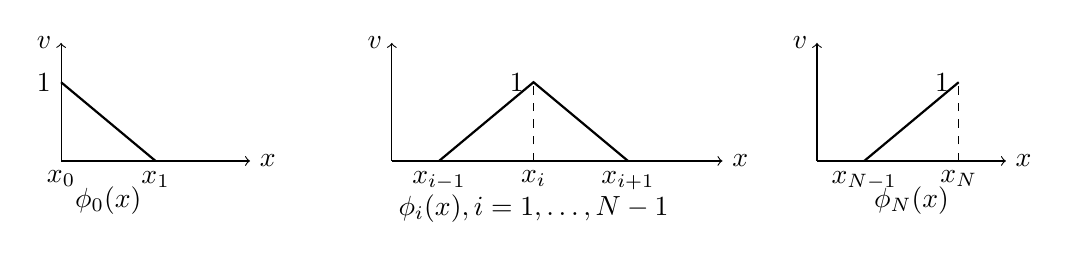
\begin{tikzpicture}[xscale=1.2, yscale=1]
  % phi_0
  \begin{scope}[shift={(0,0)}]
      \draw[->] (0,0) -- (2,0) node[right] {$x$};
      \draw[->] (0,0) -- (0,1.5) node[left] {$v$};
      \draw[thick] (0,1) node[left] {$1$} -- (1,0) node[below] {$x_1$};
      \draw[thick] (1,0) -- (1.5,0);
      \node at (0.5, -0.5) {$\phi_0(x)$};
      \node[below] at (0,0) {$x_0$};
  \end{scope}
  
  % phi_i
  \begin{scope}[shift={(3.5,0)}]
      \draw[->] (0,0) -- (3.5,0) node[right] {$x$};
      \draw[->] (0,0) -- (0,1.5) node[left] {$v$};
      \draw[thick] (0.5,0) node[below] {$x_{i-1}$} -- (1.5,1) -- (2.5,0) node[below] {$x_{i+1}$};
      \draw[dashed] (1.5,0) node[below] {$x_i$} -- (1.5,1) node[left] {$1$};
      \node at (1.5, -0.6) {$\phi_i(x), i=1,\dots,N-1$};
  \end{scope}

  % phi_N
  \begin{scope}[shift={(8,0)}]
      \draw[->] (0,0) -- (2,0) node[right] {$x$};
      \draw[->] (0,0) -- (0,1.5) node[left] {$v$};
      \draw[thick] (0.5,0) node[below] {$x_{N-1}$} -- (1.5,1);
      \draw[dashed] (1.5,0) node[below] {$x_N$} -- (1.5,1) node[left] {$1$};
      \node at (1.0, -0.5) {$\phi_N(x)$};
  \end{scope}
\end{tikzpicture}
\captionof{figure}{有限元基函数}
\end{figure}
以上分析表明 
\begin{equation*}
    U_h = \text{span}\{\phi_0, \phi_1, \dots, \phi_N\}.
\end{equation*}
再考虑 $V_h$，注意到 
\begin{equation*}
    V_h=\{v_h\in U_h:v_h(a)=0\},
\end{equation*}
我们有$\forall\, v_h\in V_h,v_h(x_0)=0$.于是
\begin{equation}
V_h = \text{span}\{\phi_1, \phi_2, \dots, \phi_N\}.
\end{equation}

\subsection{有限元方程组的形成}

\paragraph{直接法}
为了研究方便，记 $\{v\}_1 = \{v_h(x_1), \dots, v_h(x_N)\}^T$，则需找 $\{u\}_1 \in \mathbb{R}^N$ 使得：
\begin{equation*}
\begin{cases}
u_h = \sum_{i=1}^N u_i \phi_i, \\
A(u_h, v_h) = F(v_h), \quad \forall v_h \in V_h.
\end{cases}
\end{equation*}
换言之，要求成立：
\begin{equation*}
A\left(\sum_{i=1}^N u_i \phi_i, \sum_{j=1}^N v_j \phi_j\right) = \sum_{j=1}^N v_j F(\phi_j), \quad \forall \{v\}_1 \in \mathbb{R}^N,
\end{equation*}
提取系数可得：
\begin{equation*}
\sum_{i=1}^N \sum_{j=1}^N u_i v_j A(\phi_i, \phi_j) = \sum_{j=1}^N v_j F(\phi_j).
\end{equation*}
设 $\bm{A} = [a_{ij}]_{N \times N}$，其中 $a_{ij} = A(\phi_j, \phi_i)$，则上式即为 $(\bm{A}\{u\}_1, \{v\}_1) = (F, \{v\}_1)$.由此获得线性方程组 $AU = F$，式中 $U = \{u\}_1$.

\paragraph{子结构方法}
在一维情形下，有限元方法简单的原因在于我们可以通过
\begin{equation*}
    A(u_h, v_h) = (\bm{A}\{u\},\{v\})
\end{equation*}
直接得到矩阵和方程.但在高维情形下，基函数的结构会变得非常复杂，直接法不再适用.因此我们需要通过子结构方法来构造矩阵和方程.

考虑到总体变分型是由局部叠加而成：
\begin{equation}\label{eq:total_A}
A(u_h, v_h) = \sum_{i=1}^N \int_{e_i} (pu_h'v_h' + qu_h v_h)dx + \alpha u_h(b)v_h(b).
\end{equation}
(1) \textbf{单元刚度矩阵和荷载向量的计算} \\
记局部双线性型为：
\begin{align*}
A_i(u_h, v_h) &= \int_{e_i} (pu_h'v_h' + qu_h v_h)dx, \quad 1 \le i \le N-1, \\
A_N(u_h, v_h) &= \int_{e_N} (pu_h'v_h' + qu_h v_h)dx + \alpha u_h(b)v_h(b).
\end{align*}
将公式 \eqref{eq:local_basis} 中的局部基函数代入直接计算：
\begin{align*}
\int_{e_i} (pu_h'v_h' + qu_h v_h)dx &= \int_{x_{i-1}}^{x_i} \{ p(u_{i-1}N_i' + u_i M_i')(v_{i-1}N_i' + v_i M_i') \\
&\quad + q(u_{i-1}N_i + u_i M_i)(v_{i-1}N_i + v_i M_i) \} dx \\
&= ([K]_{e_i} \{u\}_{e_i}, \{v\}_{e_i}) =: (K_1^i \{u\}_{e_i}, \{v\}_{e_i}).
\end{align*}
式中 $\{v\}_{e_i} = [v_h(x_{i-1}), v_h(x_i)]^T$.

类似地，对于边界项可得：
\begin{equation*}
\alpha u_h(b)v_h(b) = \alpha u_N v_N = \left( \begin{bmatrix} 0 & 0 \\ 0 & 1 \end{bmatrix} \{u\}_{e_N}, \{v\}_{e_N} \right) =: (K_2^N \{u\}_{e_N}, \{v\}_{e_N}).
\end{equation*}

于是，
\begin{equation*}
    A_i(u_h, v_h) = (K^i \{u\}_{e_i}, \{v\}_{e_i}),
\end{equation*}
式中，当 $1 \leq i \leq N-1$ 时 $K^i = K_1^i$，而 $K^N = K_1^N + K_2^N$ 由此可得单元刚度矩阵.

再看右端，
\begin{equation}\label{eq:load_vector}
F(v_h) = \sum_{i=1}^N \int_{e_i} f v_h dx + g v_h(b),
\end{equation}
其中，
\begin{gather*}
\int_{e_i} f v_h dx = \int_{x_{i-1}}^{x_i} f (v_{i-1}N_i + v_i M_i) dx = (\{F\}_{e_i}, \{v\}_{e_i}), \\
\{F\}_{e_i} = \begin{bmatrix} \int_{x_{i-1}}^{x_i} f N_i dx \\ \int_{x_{i-1}}^{x_i} f M_i dx \end{bmatrix}, \\
\alpha v_h(b) = \left( \alpha \begin{bmatrix} 0 \\ 1 \end{bmatrix}, \{v\}_{e_N} \right).
\end{gather*}
仿上可得单元荷载向量.

\paragraph{(2) 总刚度矩阵和总荷载向量的形成}
显然，双线性型 $A_i(\cdot, \cdot)$ 是关于 $\{u\}_{e_i}$ 和 $\{v\}_{e_i}$ 局部双线性型，它自然是关于总体变量 $\{u\}$ 和 $\{v\}$ 双线性型，式中
\begin{align*}
\{u\} &= [u_h(x_0), u_h(x_1), \dots, u_h(x_N)]^T = [u_0, u_1, \dots, u_N]^T, \\
\{v\} &= [v_h(x_0), v_h(x_1), \dots, v_h(x_N)]^T = [v_0, v_1, \dots, v_N]^T.
\end{align*}
记此时相应的矩阵为 $\overline{\bm{K}}^i$.易知，该矩阵在 $(i-1, i-1)$ 位置的元素为 $\bm{K}^i$ 在位置 $(1,1)$ 的元素，在 $(i-1, i)$ 位置的元素为 $\bm{K}^i$ 在位置 $(1,2)$ 的元素，在 $(i, i-1)$ 位置的元素为 $\bm{K}^i$ 在位置 $(2,1)$ 的元素，在 $(i,i)$ 位置的元素为 $\bm{K}^i$ 在位置 $(2,2)$ 的元素，而在其他位置的元素为 0.于是，易知总刚度矩阵为
\begin{equation}
[K] = \sum_{i=1}^N \overline{\bm{K}}^i.
\end{equation}
类似可得总荷载向量 $\{F\}$.

\paragraph{(3) 约束条件的处理}
显然，
\begin{equation*}
A(u_h, v_h) = ([K]\{u\}, \{v\}),
\end{equation*}
这是不考虑 $V_h$ 中存在约束条件相应的结果.但若存在边界约束条件，例如本节介绍的例子：由 $v_h(a) = 0$ 可知 $v_0 = 0$.此时，
\begin{equation*}
A(u_h, v_h) = \left( [K] \begin{bmatrix} 0 \\ * \\ \vdots \end{bmatrix}, \begin{bmatrix} 0 \\ * \\ \vdots \end{bmatrix} \right) = (A\{u\}_1, \{v\}_1),
\end{equation*}
式中，
\begin{equation*}
[K] = \begin{bmatrix} * & \dots \\ \vdots & A \end{bmatrix}.
\end{equation*}
换言之，只需删除总刚度矩阵 $[K]$ 相应于带约束条件的节点编号对应的行和列，则可以得到有限元线性方程组对应的系数矩阵.类似可由总荷载 $[F]$ 获得有限元线性方程组对应的右端向量.

\subsection{子结构方法执行实例}

\textbf{例} 采用线性有限元方法求解以下问题：
\begin{equation}
\begin{cases}
-u''(x) = f(x), & x \in (0,1), \\
u(0) = 0, \quad u'(1) = g.
\end{cases}
\end{equation}
其中 $f(x)$ 及常数 $g$ 已知.

该问题对应的变分问题为：求 $u \in V$ 使得
\begin{equation}
A(u, v) = F(v), \quad \forall v \in V,
\end{equation}
式中
\begin{align*}
V &= \{v \in H^1(0,1) : v(0) = 0\}, \\
A(u,v) &= \int_0^1 u' v' dx, \quad F(v) = \int_0^1 f v dx + g v(1).
\end{align*}

采用 $N+1$ 个节点 $x_i$ ($i=0,1,\dots,N$) 对区间 $[0,1]$ 进行剖分：$0 = x_0 < x_1 < \dots < x_N = 1$.记 $h_j = x_j - x_{j-1}, e_j = [x_{j-1}, x_j], j=1,\dots,N$.构造有限元空间
\begin{equation*}
V_h = \{v \in C[0,1] : v|_{e_i} \in P_1(e_i), v(0) = 0\}.
\end{equation*}
有限元解为 $u_h \in V_h$，满足 $A(u_h, v_h) = F(v_h)$.

\paragraph{a. 局部刚度矩阵与局部荷载向量}
注意到：
\begin{equation*}
\int_{e_i} u' v' dx = \int_{x_{i-1}}^{x_i} \{u_{i-1}N_i + u_i M_i\}' \{v_{i-1}N_i + v_i M_i\}' dx,
\end{equation*}
其中，
\begin{equation*}
N_i = \frac{x_i - x}{h_i}, \quad M_i = \frac{x - x_{i-1}}{h_i}, \quad N_i' = -\frac{1}{h_i}, \quad M_i' = \frac{1}{h_i}.
\end{equation*}
所以，
\begin{align*}
\int_{e_i} u' v' dx &= \frac{1}{h_i^2} \int_{x_{i-1}}^{x_i} \{u_i - u_{i-1}\} \{v_i - v_{i-1}\} dx \\
&= \frac{1}{h_i} (u_i v_i - u_i v_{i-1} - u_{i-1} v_i + u_{i-1} v_{i-1}),
\end{align*}
从而局部刚度矩阵为：
\begin{equation}\label{eq:local_K}
[K]_{e_i} = \frac{1}{h_i} \begin{bmatrix} 1 & -1 \\ -1 & 1 \end{bmatrix}.
\end{equation}
若用梯形公式进行数值积分，有 $\int_{e_i} f v dx \approx \frac{1}{2} h_i [f(x_{i-1})v_{i-1} + f(x_i)v_i]$，可知：
\begin{equation}
\{F\}_{e_i} = \frac{h_i}{2} \begin{bmatrix} f(x_{i-1}) \\ f(x_i) \end{bmatrix}.
\end{equation}

\paragraph{b. 整体刚度矩阵和整体荷载的形成}
将局部矩阵扩张至 $(N+1) \times (N+1)$ 维度：
\begin{equation*}
[K]_{e_1} \to \begin{bmatrix}
\frac{1}{h_1} & -\frac{1}{h_1} & 0 & \dots & 0 \\
-\frac{1}{h_1} & \frac{1}{h_1} & 0 & \dots & 0 \\
0 & 0 & 0 & \dots & 0 \\
\vdots & \vdots & \vdots & \ddots & \vdots \\
0 & 0 & 0 & \dots & 0
\end{bmatrix}, \quad
\{F\}_{e_1} \to \frac{h_1}{2} \begin{bmatrix} f(x_0) \\ f(x_1) \\ 0 \\ \vdots \\ 0 \end{bmatrix}.
\end{equation*}

\begin{equation*}
[K]_{e_2} \to \begin{bmatrix}
0 & 0 & 0 & \dots & 0 \\
0 & \frac{1}{h_2} & -\frac{1}{h_2} & \dots & 0 \\
0 & -\frac{1}{h_2} & \frac{1}{h_2} & \dots & 0 \\
\vdots & \vdots & \vdots & \ddots & \vdots \\
0 & 0 & 0 & \dots & 0
\end{bmatrix}, \quad
\{F\}_{e_2} \to \frac{h_2}{2} \begin{bmatrix} 0 \\ f(x_1) \\ f(x_2) \\ 0 \\ \vdots \\ 0 \end{bmatrix}.
\end{equation*}

其余均类似，且边界荷载向量 $\{F\}_{e_N}$ 最后分量包含常数 $g$：
\begin{equation*}
\{F\}_{e_N} \to \begin{bmatrix} 0 \\ \vdots \\ 0 \\ \frac{h_N}{2} f(x_{N-1}) \\ \frac{h_N}{2} f(x_N) + g \end{bmatrix}.
\end{equation*}

全部叠加起来有总体刚度矩阵和总体荷载向量：
\begin{equation}
[K] = \begin{bmatrix}
\frac{1}{h_1} & -\frac{1}{h_1} & & & & \\
-\frac{1}{h_1} & \frac{1}{h_1} + \frac{1}{h_2} & -\frac{1}{h_2} & & & \\
& -\frac{1}{h_2} & \frac{1}{h_2} + \frac{1}{h_3} & -\frac{1}{h_3} & & \\
& & \ddots & \ddots & \ddots & \\
& & & -\frac{1}{h_{N-1}} & \frac{1}{h_{N-1}} + \frac{1}{h_N} & -\frac{1}{h_N} \\
& & & & -\frac{1}{h_N} & \frac{1}{h_N}
\end{bmatrix}_{(N+1) \times (N+1)}
\end{equation}
\begin{equation}
\{F\} = \begin{bmatrix}
f(x_0) \frac{h_1}{2} \\
f(x_1) \frac{h_1 + h_2}{2} \\
f(x_2) \frac{h_2 + h_3}{2} \\
\vdots \\
f(x_{N-1}) \frac{h_{N-1} + h_N}{2} \\
f(x_N) \frac{h_N}{2} + g
\end{bmatrix}_{(N+1) \times 1}
\end{equation}

\paragraph{c. 约束条件的处理}
将边界条件 $u(0)=0$ 对应的行列（即第一行和第一列）去掉，得最终的系数矩阵 $A$ 和右端向量 $b$：
\begin{equation}
A = \begin{bmatrix}
\frac{1}{h_1} + \frac{1}{h_2} & -\frac{1}{h_2} & & & \\
-\frac{1}{h_2} & \frac{1}{h_2} + \frac{1}{h_3} & -\frac{1}{h_3} & & \\
& \ddots & \ddots & \ddots & \\
& & -\frac{1}{h_{N-1}} & \frac{1}{h_{N-1}} + \frac{1}{h_N} & -\frac{1}{h_N} \\
& & & -\frac{1}{h_N} & \frac{1}{h_N}
\end{bmatrix}_{N \times N}
\end{equation}
\begin{equation}
b = \begin{bmatrix}
\frac{f(x_1)}{2}(h_1 + h_2) \\
\vdots \\
\frac{f(x_{N-1})}{2}(h_{N-1} + h_N) \\
\frac{f(x_N)}{2}h_N + g
\end{bmatrix}_{N \times 1}
\end{equation}
最后求解线性代数方程组 $AU = b$，获得 $U = [u_1, u_2, \dots, u_N]^T$，由此可得近似解 $u_h = \sum_{i=1}^N u_i \phi_i$.

\subsection{子结构方法 (续)}

再看右端，
\begin{equation}\label{eq:load_vector}
F(v_h) = \sum_{i=1}^N \int_{e_i} f v_h dx + g v_h(b),
\end{equation}
其中，
\begin{align*}
\int_{e_i} f v_h dx &= \int_{x_{i-1}}^{x_i} f (v_{i-1}N_i + v_i M_i) dx = (\{F\}_{e_i}, \{v\}_{e_i}), \\
\{F\}_{e_i} &= \begin{bmatrix} \int_{x_{i-1}}^{x_i} f N_i dx \\ \int_{x_{i-1}}^{x_i} f M_i dx \end{bmatrix}, \\
\alpha v_h(b) &= \left( \alpha \begin{bmatrix} 0 \\ 1 \end{bmatrix}, \{v\}_{e_N} \right).
\end{align*}
仿上可得单元荷载向量.

\paragraph{(2) 总刚度矩阵和总荷载向量的形成}
显然，双线性型 $A_i(\cdot, \cdot)$ 是关于 $\{u\}_{e_i}$ 和 $\{v\}_{e_i}$ 局部双线性型，它自然是关于总体变量 $\{u\}$ 和 $\{v\}$ 双线性型，式中
\begin{align*}
\{u\} &= [u_h(x_0), u_h(x_1), \dots, u_h(x_N)]^T = [u_0, u_1, \dots, u_N]^T, \\
\{v\} &= [v_h(x_0), v_h(x_1), \dots, v_h(x_N)]^T = [v_0, v_1, \dots, v_N]^T.
\end{align*}
记此时相应的矩阵为 $\overline{K}^i$.易知，该矩阵在 $(i-1, i-1)$ 位置的元素为 $K^i$ 在位置 $(1,1)$ 的元素，在 $(i-1, i)$ 位置的元素为 $K^i$ 在位置 $(1,2)$ 的元素，在 $(i, i-1)$ 位置的元素为 $K^i$ 在位置 $(2,1)$ 的元素，在 $(i,i)$ 位置的元素为 $K^i$ 在位置 $(2,2)$ 的元素，而在其他位置的元素为 0.于是，易知总刚度矩阵为
\begin{equation}
[K] = \sum_{i=1}^N \overline{K}^i.
\end{equation}
类似可得总荷载向量 $\{F\}$.

\paragraph{(3) 约束条件的处理}
显然，
\begin{equation*}
A(u_h, v_h) = ([K]\{u\}, \{v\}),
\end{equation*}
这是不考虑 $V_h$ 中存在约束条件相应的结果.但若存在边界约束条件，例如本节介绍的例子：由 $v_h(a) = 0$ 可知 $v_0 = 0$.此时，
\begin{equation*}
A(u_h, v_h) = \left( [K] \begin{bmatrix} 0 \\ * \\ \vdots \end{bmatrix}, \begin{bmatrix} 0 \\ * \\ \vdots \end{bmatrix} \right) = (A\{u\}_1, \{v\}_1),
\end{equation*}
式中，
\begin{equation*}
[K] = \begin{bmatrix} * & \dots \\ \vdots & A \end{bmatrix}.
\end{equation*}
换言之，只需删除总刚度矩阵 $[K]$ 相应于带约束条件的节点编号对应的行和列，则可以得到有限元线性方程组对应的系数矩阵.类似可由总荷载 $[F]$ 获得有限元线性方程组对应的右端向量.

\subsection{子结构方法执行实例}

\textbf{例} 采用线性有限元方法求解以下问题：
\begin{equation}
\begin{cases}
-u''(x) = f(x), & x \in (0,1), \\
u(0) = 0, \quad u'(1) = g.
\end{cases}
\end{equation}
其中 $f(x)$ 及常数 $g$ 已知.

该问题对应的变分问题为：求 $u \in V$ 使得
\begin{equation}
A(u, v) = F(v), \quad \forall v \in V,
\end{equation}
式中
\begin{align*}
V &= \{v \in H^1(0,1) : v(0) = 0\}, \\
A(u,v) &= \int_0^1 u' v' dx, \quad F(v) = \int_0^1 f v dx + g v(1).
\end{align*}

采用 $N+1$ 个节点 $x_i$ ($i=0,1,\dots,N$) 对区间 $[0,1]$ 进行剖分：$0 = x_0 < x_1 < \dots < x_N = 1$.记 $h_j = x_j - x_{j-1}, e_j = [x_{j-1}, x_j], j=1,\dots,N$.构造有限元空间
\begin{equation*}
V_h = \{v \in C[0,1] : v|_{e_i} \in P_1(e_i), v(0) = 0\}.
\end{equation*}
有限元解为 $u_h \in V_h$，满足 $A(u_h, v_h) = F(v_h)$.

\paragraph{a. 局部刚度矩阵与局部荷载向量}
注意到：
\begin{equation*}
\int_{e_i} u' v' dx = \int_{x_{i-1}}^{x_i} \{u_{i-1}N_i + u_i M_i\}' \{v_{i-1}N_i + v_i M_i\}' dx,
\end{equation*}
其中，
\begin{equation*}
N_i = \frac{x_i - x}{h_i}, \quad M_i = \frac{x - x_{i-1}}{h_i}, \quad N_i' = -\frac{1}{h_i}, \quad M_i' = \frac{1}{h_i}.
\end{equation*}
所以，
\begin{align*}
\int_{e_i} u' v' dx &= \frac{1}{h_i^2} \int_{x_{i-1}}^{x_i} \{u_i - u_{i-1}\} \{v_i - v_{i-1}\} dx \\
&= \frac{1}{h_i} (u_i v_i - u_i v_{i-1} - u_{i-1} v_i + u_{i-1} v_{i-1}),
\end{align*}
从而局部刚度矩阵为：
\begin{equation}\label{eq:local_K}
[K]_{e_i} = \frac{1}{h_i} \begin{bmatrix} 1 & -1 \\ -1 & 1 \end{bmatrix}.
\end{equation}
若用梯形公式进行数值积分，有 $\int_{e_i} f v dx \approx \frac{1}{2} h_i [f(x_{i-1})v_{i-1} + f(x_i)v_i]$，可知：
\begin{equation}
\{F\}_{e_i} = \frac{h_i}{2} \begin{bmatrix} f(x_{i-1}) \\ f(x_i) \end{bmatrix}.
\end{equation}

\paragraph{b. 整体刚度矩阵和整体荷载的形成}
将局部矩阵扩张至 $(N+1) \times (N+1)$ 维度：
\begin{equation*}
[K]_{e_1} \to \begin{bmatrix}
\frac{1}{h_1} & -\frac{1}{h_1} & 0 & \dots & 0 \\
-\frac{1}{h_1} & \frac{1}{h_1} & 0 & \dots & 0 \\
0 & 0 & 0 & \dots & 0 \\
\vdots & \vdots & \vdots & \ddots & \vdots \\
0 & 0 & 0 & \dots & 0
\end{bmatrix}, \quad
\{F\}_{e_1} \to \frac{h_1}{2} \begin{bmatrix} f(x_0) \\ f(x_1) \\ 0 \\ \vdots \\ 0 \end{bmatrix}.
\end{equation*}

\begin{equation*}
[K]_{e_2} \to \begin{bmatrix}
0 & 0 & 0 & \dots & 0 \\
0 & \frac{1}{h_2} & -\frac{1}{h_2} & \dots & 0 \\
0 & -\frac{1}{h_2} & \frac{1}{h_2} & \dots & 0 \\
\vdots & \vdots & \vdots & \ddots & \vdots \\
0 & 0 & 0 & \dots & 0
\end{bmatrix}, \quad
\{F\}_{e_2} \to \frac{h_2}{2} \begin{bmatrix} 0 \\ f(x_1) \\ f(x_2) \\ 0 \\ \vdots \\ 0 \end{bmatrix}.
\end{equation*}

其余均类似，且边界荷载向量 $\{F\}_{e_N}$ 最后分量包含常数 $g$：
\begin{equation*}
\{F\}_{e_N} \to \begin{bmatrix} 0 \\ \vdots \\ 0 \\ \frac{h_N}{2} f(x_{N-1}) \\ \frac{h_N}{2} f(x_N) + g \end{bmatrix}.
\end{equation*}

全部叠加起来有总体刚度矩阵和总体荷载向量：
\begin{equation}
[K] = \begin{bmatrix}
\frac{1}{h_1} & -\frac{1}{h_1} & & & & \\
-\frac{1}{h_1} & \frac{1}{h_1} + \frac{1}{h_2} & -\frac{1}{h_2} & & & \\
& -\frac{1}{h_2} & \frac{1}{h_2} + \frac{1}{h_3} & -\frac{1}{h_3} & & \\
& & \ddots & \ddots & \ddots & \\
& & & -\frac{1}{h_{N-1}} & \frac{1}{h_{N-1}} + \frac{1}{h_N} & -\frac{1}{h_N} \\
& & & & -\frac{1}{h_N} & \frac{1}{h_N}
\end{bmatrix}_{(N+1) \times (N+1)}
\end{equation}
\begin{equation}
\{F\} = \begin{bmatrix}
f(x_0) \frac{h_1}{2} \\
f(x_1) \frac{h_1 + h_2}{2} \\
f(x_2) \frac{h_2 + h_3}{2} \\
\vdots \\
f(x_{N-1}) \frac{h_{N-1} + h_N}{2} \\
f(x_N) \frac{h_N}{2} + g
\end{bmatrix}_{(N+1) \times 1}
\end{equation}

\paragraph{c. 约束条件的处理}
将边界条件 $u(0)=0$ 对应的行列（即第一行和第一列）去掉，得最终的系数矩阵 $A$ 和右端向量 $b$：
\begin{equation}
A = \begin{bmatrix}
\frac{1}{h_1} + \frac{1}{h_2} & -\frac{1}{h_2} & & & \\
-\frac{1}{h_2} & \frac{1}{h_2} + \frac{1}{h_3} & -\frac{1}{h_3} & & \\
& \ddots & \ddots & \ddots & \\
& & -\frac{1}{h_{N-1}} & \frac{1}{h_{N-1}} + \frac{1}{h_N} & -\frac{1}{h_N} \\
& & & -\frac{1}{h_N} & \frac{1}{h_N}
\end{bmatrix}_{N \times N}
\end{equation}
\begin{equation}
b = \begin{bmatrix}
\frac{f(x_1)}{2}(h_1 + h_2) \\
\vdots \\
\frac{f(x_{N-1})}{2}(h_{N-1} + h_N) \\
\frac{f(x_N)}{2}h_N + g
\end{bmatrix}_{N \times 1}
\end{equation}
最后求解线性代数方程组 $AU = b$，获得 $U = [u_1, u_2, \dots, u_N]^T$，由此可得近似解 $u_h = \sum_{i=1}^N u_i \phi_i$.

\section{一维线性有限元方法的理论分析}

\subsection{可解性分析}

一个自然的问题是有限元线性方程组
\begin{equation*}
\boldsymbol{A}\boldsymbol{x} = \boldsymbol{b}
\end{equation*}
是否唯一可解，即 $\boldsymbol{A}$ 是否可逆？

\begin{theorem}[对称正定性][thm:spd-matrix]
$\boldsymbol{A}$ 为对称正定阵.
\end{theorem}

\begin{proof}
因 $a_{ij} = a(\phi_j, \phi_i)$，而 $A(u,v) = A(v,u)$，故 $a_{ij} = a_{ji}$，故 $\boldsymbol{A}$
的对称性显然成立.下证正定性.对任意的 $\boldsymbol{v} = [v_1,\cdots,v_N]^{\mathsf{T}} \in
\mb{R}^N$ 可构造函数 $v_h = \sum_{i=1}^N v_i\phi_i(x)$.易知
\begin{equation*}
A(v_h, v_h) = (\boldsymbol{A}\boldsymbol{v}, \boldsymbol{v}).
\end{equation*}
注意到
\begin{align*}
A(v_h, v_h) &= \sum_{i=1}^{N} \int_{e_i}(pv_h' v_h' + qv_h v_h)\d x + \alpha v_h(b) v_h(b) \\
&\geq \int_a^b p(v_h')^2 \d x \geq p_0 \int_a^b (v_h')^2 \d x \geq 0.
\end{align*}
等号成立至少应成立
\begin{equation*}
\int_a^b (v_h')^2 \d x = 0,
\end{equation*}
即
\begin{equation*}
v_h'\big|_{e_i} = 0.
\end{equation*}
这说明 $v_h$ 在每一个单元上都为常数，而 $v_h$ 又在 $[a,b]$ 上连续，故
\begin{equation*}
v_h \equiv C = \text{常数},
\end{equation*}
由 $v_h(a) = 0$ 可得 $C = 0$.上面的分析表明，$(\boldsymbol{A}\boldsymbol{v}, \boldsymbol{v}) \geq
 0$，且等号成立当且仅当 $\boldsymbol{v} = \boldsymbol{0}$.
\end{proof}

\subsection{收敛性分析}

在空间 $V$ 中引入范数
\begin{equation*}
\norm{v}_1 = \ab(\int_a^b (v')^2 \d x)^{1/2}, \quad v \in V.
\end{equation*}

\begin{lemma}[强制性有界性][lem:continuity-coercivity]
存在正常数 $M_1, M_2$，使得
\begin{equation}\label{eq:coercivity}
M_1 \norm{v}_1^2 \leq A(v,v), \quad v \in V,
\end{equation}
\begin{equation}\label{eq:continuity}
|A(u,v)| \leq M_2 \norm{u}_1 \norm{v}_1, \quad u, v \in V.
\end{equation}
\end{lemma}

\begin{proof}
第一步：给出估计式 (\ref{eq:coercivity}).对任意 $v \in V$，
\begin{align*}
A(v,v) &= \int_a^b (pv'^2 + qv^2)\d x + \alpha v^2(b) \\
&\geq p_0 \int_a^b v'^2 \d x = p_0 \norm{v}_1^2.
\end{align*}
取 $M_1 = p_0$，即证得 (\ref{eq:coercivity}).\par
第二步：给出 $V$ 中 $\norm{\cdot}_0$, $\norm{\cdot}_{0,\infty}$ 和 $\norm{\cdot}_1$
之间的关系.直接计算有
\begin{align*}
\norm{v}_0^2 &= \int_a^b v^2(x)\d x = \int_a^b \ab(\int_a^x v'(s)\d s)^2 \d x \\
&\leq \int_a^b \ab(\int_a^x 1\d s)\ab(\int_a^x |v'(s)|^2 \d s) \d x \\
&\leq \int_a^b (x-a)\d x \int_a^b |v'(s)|^2 \d s \\
&= \frac{1}{2}(b-a)^2 \norm{v}_1^2,
\end{align*}
故
\begin{equation}\label{eq:l2-bound}
\norm{v}_0 \leq c_1 \norm{v}_1, \quad v \in V,
\end{equation}
式中 $c_1 = \frac{\sqrt{2}}{2}(b-a)$.类似地，可知
\begin{equation}\label{eq:linf-bound}
\norm{v}_{0,\infty} \leq c_2 \norm{v}_1, \quad v \in V,
\end{equation}
式中 $c_2 = \sqrt{b-a}$.\par
第三步：给出估计式 (\ref{eq:continuity}).记 $M = \max_{a \leq x \leq b} \max(|p(x)|,
|q(x)|)$.对任意的 $u, v \in V$，由 (\ref{eq:l2-bound})--(\ref{eq:linf-bound}) 和 Cauchy-Schwarz
不等式可得
\begin{align*}
A(u,v) &= \int_a^b (pu'v' + quv)\d x + \alpha u(b)v(b) \\
&\leq M\int_a^b |u'v'|\d x + M\int_a^b |uv|\d x + \alpha\, |u(b)|\,|v(b)| \\
&\leq M\norm{u'}_0 \norm{v'}_0 + M\norm{u}_0 \norm{v}_0 + \alpha\, |u(b)|\,|v(b)| \\
&\leq (M + Mc_1^2 + \alpha c_2^2)\norm{u}_1\norm{v}_1 = M_2 \norm{u}_1\norm{v}_1.
\end{align*}
式中，$M_2 = M + Mc_1^2 + \alpha c_2^2$.
\end{proof}

% ---------- 过渡 -----------
上述引理表明双线性型 $A(\cdot,\cdot)$ 在 $\norm{\cdot}_1$ 范数下既是强制的又是有界的，这为后续的
C\'ea 引理提供了必要的前提条件.
% ---------- 过渡 -----------

\begin{lemma}[C\'ea 引理][lem:cea]
设 $u$ 为原问题之解，$u_h$ 为有限元解，则
\begin{equation*}
\norm{u - u_h}_1 \leq C \cdot \inf_{v \in V_h} \norm{u - v}_1,
\end{equation*}
式中及后文中，$C$ 均为一与 $h$ 无关的生成常数，在不同的地方可取不同值.
\end{lemma}

\begin{proof}
由 $V_h \subset V$ 知 $\forall\, v_h \in V_h$，易知成立如下 Galerkin 正交性
\begin{equation*}
A(u - u_h, v_h) = 0, \quad v_h \in V_h,
\end{equation*}
于是
\begin{equation*}
A(u - u_h, u - u_h) = A(u - u_h, u - v_h), \quad v_h \in V_h.
\end{equation*}
而由\cref{lem:continuity-coercivity}，等式左边 $\geq M_1 \norm{u - u_h}_1^2$，等式右边 $\leq M_2
\norm{u - u_h}_1 \cdot \norm{u - v_h}_1$，所以
\begin{equation*}
\norm{u - u_h}_1 \leq \frac{M_2}{M_1} \norm{u - v_h}_1.
\end{equation*}
再由 $v_h \in V_h$ 的任意性立知结果.
\end{proof}

现在的问题是如何选取 $v$.显然 $v$ 的信息由 $v$ 在单元顶点 $x_0, x_1, \cdots, x_N$
上的值完全确定，自然地要求：
\begin{equation*}
v(x_i) = u(x_i), \quad i = 0, 1, 2, \cdots, N.
\end{equation*}
因此，取 $v$ 为 $u$ 的连续分段线性插值函数，记之为 $\Pi_h u$.这样，问题的关键转化为如何估计
$\norm{u - \Pi_h u}_1$.

\begin{lemma}[插值误差估计][lem:interpolation]
设 $u \in V \cap C^2[a,b]$，$\Pi_h$ 为连续分段线性插值算子，则成立
\begin{equation*}
\norm{u - \Pi_h u}_1 \leq h |u|_2,
\end{equation*}
式中，
\begin{equation*}
|u|_2 = \ab(\int_a^b |u''|^2 \d x)^{\frac{1}{2}},
\end{equation*}
而 $h$ 为网格剖分的直径.
\end{lemma}

\begin{proof}
根据插值算子的定义，直接计算并利用 Lagrange 中值定理有
\begin{align*}
\norm{u - \Pi_h u}_1^2 &= \int_a^b (u - \Pi_h u)'^2 \d x = \sum_{i=1}^N \int_{x_{i-1}}^{x_i} (u -
 \Pi_h u)'^2 \d x \\
&= \sum_{i=1}^N \int_{x_{i-1}}^{x_i} \ab(u'(x) - \frac{u(x_i) - u(x_{i-1})}{x_i - x_{i-1}})^2 \d
x \\
&= \sum_{i=1}^N \int_{x_{i-1}}^{x_i} (u'(x) - u'(\xi_i))^2 \d x, \\
&= \sum_{i=1}^N \int_{x_{i-1}}^{x_i} (u'(x) - u'(\xi_i))^2 \d x,
\end{align*}
式中，$\xi_i \in (x_{i-1}, x_i)$.于是
\begin{align*}
\norm{u - \Pi_h u}_1^2 &= \sum_{i=1}^N \int_{x_{i-1}}^{x_i} \ab(\int_{\xi_i}^x u''(s)\d s)^2 \d x
 \\
&\leq \sum_{i=1}^N \int_{x_{i-1}}^{x_i} \left\{\left|\int_{\xi_i}^x 1^2 \d s\right|
\left|\int_{\xi_i}^x u''^2 \d s\right|\right\} \d x \\
&\leq \sum_{i=1}^N \int_{x_{i-1}}^{x_i} u''^2 \d x \int_{x_{i-1}}^{x_i} |x - \xi_i| \d x \\
&\leq h^2 \sum_{i=1}^N \int_{x_{i-1}}^{x_i} (u'')^2 \d x = h^2 |u|_2.
\end{align*}
\end{proof}

% ---------- 过渡 -----------
结合 C\'ea 引理与插值误差估计，立即得到有限元解的一阶收敛性.
% ---------- 过渡 -----------

\begin{theorem}[误差估计][thm:error-estimate]
有限元解 $u_h$ 满足误差估计
\begin{equation*}
\norm{u - u_h}_1 \leq C h |u|_2,
\end{equation*}
式中，$C$ 是与 $h$ 无关的常数.
\end{theorem}

\begin{proof}
由\cref{lem:cea} 和\cref{lem:interpolation} 即知.
\end{proof}

\section{二维问题的有限元方法---线性元}

\subsection{问题描述与变分原理}

考虑问题
\begin{equation*}
\begin{cases}
-\Delta u = f, & (x,y) \in \Omega, \\
\partial_n u + \alpha u = g, & (x,y) \in \partial\Omega.
\end{cases}
\end{equation*}
假设 $\alpha(x,y) \ge 0$，且 $\alpha(x,y)$ 不恒为 $0$，唯一性由极值原理易证.\par

% ---------- 过渡 -----------
上述问题可转化为如下 Galerkin 变分形式.
% ---------- 过渡 -----------

求 $u \in V$ 使
\begin{equation*}
A(u,v) = F(v), \quad v \in V,
\end{equation*}
其中
\begin{align*}
A(u,v) &= \int_\Omega \nabla u \cdot \nabla v \, \mathrm{d}x\mathrm{d}y + \int_{\partial\Omega} \alpha u v \, \mathrm{d}s, \\
F(v) &= \int_\Omega f v \, \mathrm{d}x\mathrm{d}y + \int_{\partial\Omega} g v \, \mathrm{d}s.
\end{align*}

对于纯粹 Neumann 边界条件的问题
\begin{equation*}
\begin{cases}
-\Delta u = f, & (x,y) \in \Omega, \\
\partial_n u = g, & (x,y) \in \partial\Omega,
\end{cases}
\end{equation*}
其解不一定存在，要有解则应满足相容性条件
\begin{equation*}
\int_\Omega (-\Delta u) \cdot 1 \, \mathrm{d}x\mathrm{d}y = \int_\Omega f \, \mathrm{d}x\mathrm{d}y,
\end{equation*}
即
\begin{equation*}
\int_\Omega f \, \mathrm{d}x\mathrm{d}y + \int_{\partial\Omega} g \, \mathrm{d}s = 0.
\end{equation*}
该条件是问题有解的必要条件，实际上也是充分条件.\par

\subsection{单元划分及试探函数空间的形成}

为研究方便，设 $\Omega$ 为平面多角形区域，首先对区域 $\Omega$ 进行三角剖分，满足：
\begin{enumerate}
\item 任一三角形单元只能与相邻三角形单元共边或共顶点；
\item 每一个三角形单元不可太尖或太钝，大小亦不可相差太大；
\item 多角形区域的角点均应为单元顶点；
\item 三角形单元充满整体多角形区域.
\end{enumerate}

\begin{itemize}
\item 单元编号：设有 $NE$ 个单元，记为 $e_k, k=1,2,\cdots,NE$.
\item 顶点编号：设有 $NP$ 个顶点，记为 $P_i = (x_i, y_i), i=1,2,\cdots,NP$.
\end{itemize}

\begin{tikzpicture}[
    scale=0.8,
    line width=0.8pt, % 较粗的线条，贴合原图风格
    % 定义节点样式为原图中的小十字 (+)
    cross/.style={cross out, draw=black, minimum size=3pt, inner sep=0pt, outer sep=0pt, line width=0.6pt}
]

% 设置随机种子以保证每次编译生成的网格形状一致
% 你可以修改这个数字 (例如换成 42 或 100) 来生成不同形态的网格
\pgfmathsetseed{15}

% 定义网格的列数和行数
\def\cols{8}
\def\rows{6}

% 1. 生成带有随机扰动（坐标偏移）的顶点
\foreach \x in {0,...,\cols} {
    \foreach \y in {0,...,\rows} {
        % 计算偏移量 (0.35 控制不规则变形的程度)
        \pgfmathsetmacro{\dx}{0.35*(rand)}
        \pgfmathsetmacro{\dy}{0.35*(rand)}
        \coordinate (n-\x-\y) at (\x + \dx, \y + \dy);
    }
}

% 2. 绘制网格连线 (水平、垂直及对角线形成三角形)
\foreach \x in {0,...,\cols} {
    \foreach \y in {0,...,\rows} {
        % 绘制水平边缘
        \ifnum\x<\cols
            \pgfmathtruncatemacro{\nextx}{\x+1}
            \draw (n-\x-\y) -- (n-\nextx-\y);
        \fi
        % 绘制垂直边缘
        \ifnum\y<\rows
            \pgfmathtruncatemacro{\nexty}{\y+1}
            \draw (n-\x-\y) -- (n-\x-\nexty);
        \fi
        % 绘制对角边缘构成三角形
        \ifnum\x<\cols
            \ifnum\y<\rows
                \pgfmathtruncatemacro{\nextx}{\x+1}
                \pgfmathtruncatemacro{\nexty}{\y+1}
                % 使用交替或随机的对角线使网格看起来更自然
                \pgfmathparse{mod(\x+\y, 2) == 0 ? 1 : 0}
                \ifnum\pgfmathresult=1
                    \draw (n-\x-\y) -- (n-\nextx-\nexty);
                \else
                    \draw (n-\x-\nexty) -- (n-\nextx-\y);
                \fi
            \fi
        \fi
    }
}

% 3. 在所有顶点处绘制十字标记 (+)
\foreach \x in {0,...,\cols} {
    \foreach \y in {0,...,\rows} {
        \node[cross] at (n-\x-\y) {};
    }
}

\end{tikzpicture}

\begin{definition}[有限元空间][def:fem-space]
\colorbf{有限元空间} $U_h$ 为基于以上三角单元剖分的连续分片线性函数全体所构成的有限维空间（$\dim U_h = NP$）.
\end{definition}
下面是 $v \in U_h$ 的具体结构：\par
(1) 从整体看，当 $\phi_i$ 为在顶点 $P_i$ 处取值为 $1$，其他顶点处取值为 $0$ 的分片连续函数，$i=1,2,\cdots,NP$ 时，$v = \sum_{i=1}^{NP} v(P_i)\phi_i$. 显然 $\phi_i$ 的支集很小，为山形函数.\par
(2) 从局部看，考察 $v$ 在任一单元 $e$ 上的具体形式. 设 $e = P_iP_jP_m$（逆时间方向），$v|_e = ax + by + c$，满足条件：
\begin{equation*}
\begin{aligned}
ax_i + by_i + c &= v(P_i) =: v_i, \\
ax_j + by_j + c &= v(P_j) =: v_j, \\
ax_m + by_m + c &= v(P_m) =: v_m.
\end{aligned}
\end{equation*}
\begin{figure}[h]
\centering
\begin{tikzpicture}[scale=1.5, join=round, cap=round]

    % ====================
    % 左侧图形: 有限元网格及形函数
    % ====================
    % 中心节点
    \coordinate (C) at (0,0);

    % 阴影区域（支撑域）内圈节点
    \coordinate (N1) at (-0.6, 0.5);
    \coordinate (N2) at (0.3, 0.7);
    \coordinate (N3) at (0.9, 0.1);
    \coordinate (N4) at (0.7, -0.4);
    \coordinate (N5) at (-0.1, -0.6);
    \coordinate (N6) at (-0.7, -0.2);

    % 外圈节点
    \coordinate (O1) at (-0.1, 1.3);
    \coordinate (O2) at (-1.3, 0.4);
    \coordinate (O3) at (-1.1, -0.8);
    \coordinate (O4) at (0.2, -1.2);
    \coordinate (O5) at (1.0, -0.8);

    % 绘制阴影填充
    \fill[pattern=north east lines, pattern color=black!60]
        (N1) -- (N2) -- (N3) -- (N4) -- (N5) -- (N6) -- cycle;

    % 绘制阴影区域的边界和内部连线
    \draw (N1) -- (N2) -- (N3) -- (N4) -- (N5) -- (N6) -- cycle;
    \foreach \i in {1,...,6} {
        \draw (C) -- (N\i);
    }

    % 绘制外围边界轮廓
    \draw (O1) -- (O2) -- (O3) -- (O4) -- (O5) -- (N3) -- (N2) -- cycle;

    % 绘制外围内部网格线
    \draw (O1) -- (N1);
    \draw (O2) -- (N1);
    \draw (O2) -- (N6);
    \draw (O3) -- (N6);
    \draw (O3) -- (N5);
    \draw (O4) -- (N5);
    \draw (O4) -- (N4);
    \draw (O5) -- (N4);

    % 绘制形函数峰值点及虚线轮廓
    \coordinate (P) at (0.3, 1.2);
    \foreach \i in {1,...,6} {
        \draw[densely dashed] (P) -- (N\i);
    }
    % 中心向上的虚线指示箭头
    \draw[densely dashed, -latex] (C) -- (P);

    % ====================
    % 右侧图形: 单个二维三角形单元
    % ====================
    \begin{scope}[shift={(2.5, 0)}]
        % 坐标系
        \coordinate (Origin) at (0,0);
        \draw[-latex] (Origin) node[below left] {$O$} -- (0.8,0) node[right] {$x$};
        \draw[-latex] (Origin) -- (0,0.8) node[left] {$y$};

        % 三角形单元的三个顶点
        \coordinate (M) at (1.2, -0.6);
        \coordinate (I) at (3.5, 0);
        \coordinate (J) at (2.0, 1.3);

        % 绘制三角形并标注节点
        \draw[thick] (M) node[below left] {$m$}
                  -- (I) node[right] {$i$}
                  -- (J) node[above left] {$j$}
                  -- cycle;

        % 单元标识 e
        \node at (2.2, 0.2) {$e$};
    \end{scope}

\end{tikzpicture}
\end{figure}


上即
\begin{equation*}
\begin{bmatrix}
x_i & y_i & 1 \\
x_j & y_j & 1 \\
x_m & y_m & 1
\end{bmatrix}
\begin{bmatrix}
a \\ b \\ c
\end{bmatrix}
=
\begin{bmatrix}
v_i \\ v_j \\ v_m
\end{bmatrix}.
\end{equation*}

记
\begin{equation*}
\triangle_e = \frac{1}{2}
\begin{vmatrix}
x_i & y_i & 1 \\
x_j & y_j & 1 \\
x_m & y_m & 1
\end{vmatrix}
\end{equation*}
为三角形 $e$ 的面积，由 Cramer 法则可求得
\begin{equation*}
a = \frac{1}{2\triangle_e}\sum_{l=i,j,m}\bar{a}_l v_l, \quad
b = \frac{1}{2\triangle_e}\sum_{l=i,j,m}\bar{b}_l v_l, \quad
c = \frac{1}{2\triangle_e}\sum_{l=i,j,m}\bar{c}_l v_l,
\end{equation*}
从而有
\begin{align*}
v|_e &= \frac{1}{2\triangle_e}(\bar{a}_i v_i + \bar{a}_j v_j + \bar{a}_m v_m)x + \frac{1}{2\triangle_e}(\bar{b}_i v_i + \bar{b}_j v_j + \bar{b}_m v_m)y \\
&\quad + \frac{1}{2\triangle_e}(\bar{c}_i v_i + \bar{c}_j v_j + \bar{c}_m v_m) \\
&= N_i v_i + N_j v_j + N_m v_m,
\end{align*}
式中，$N_i, N_j, N_m$ 为线性基函数.\par

\begin{equation*}
\begin{cases}
N_i = \dfrac{1}{2\triangle_e}(\bar{a}_i x + \bar{b}_i y + \bar{c}_i), \\[6pt]
N_j = \dfrac{1}{2\triangle_e}(\bar{a}_j x + \bar{b}_j y + \bar{c}_j), \\[6pt]
N_m = \dfrac{1}{2\triangle_e}(\bar{a}_m x + \bar{b}_m y + \bar{c}_m).
\end{cases}
\end{equation*}

显然，它们满足性质
\begin{equation*}
\begin{cases}
N_i + N_j + N_m = 1, \\
x_i N_i + x_j N_j + x_m N_m = x, \\
y_i N_i + y_j N_j + y_m N_m = y,
\end{cases}
\end{equation*}
且
\begin{equation*}
N_l(P_k) = \delta_{lk} =
\begin{cases}
1, & l = k, \\
0, & l \ne k.
\end{cases}
\end{equation*}

为了方便，重新记：$N_k := a_k x + b_k y + c_k, k = i,j,m$，其中
\begin{equation*}
a_k = \frac{1}{2\triangle_e}\bar{a}_k, \quad
b_k = \frac{1}{2\triangle_e}\bar{b}_k, \quad
c_k = \frac{1}{2\triangle_e}\bar{c}_k.
\end{equation*}

\subsection{有限元方程的形成}

在一维问题中，我们已经给出了如何由 $A(u_h, v_h) = F(v_h)$ 获得线性方程组 $A\boldsymbol{x} = \boldsymbol{b}$ 的子结构方法，该方法同样适用于二维情形，此时
\begin{equation}
A(u_h, v_h) = \sum_{n=1}^{NE}\int_{e_n} \nabla u_h \cdot \nabla v_h \, \mathrm{d}x\mathrm{d}y + \int_{\partial\Omega} \alpha u_h(s)v_h(s) \, \mathrm{d}s, \label{eq:Ahuhvh}
\end{equation}
\begin{equation}
F(v_h) = \sum_{n=1}^{NE}\int_{e_n} f v_h \, \mathrm{d}x\mathrm{d}y + \int_{\partial\Omega} g(s)v_h(s) \, \mathrm{d}s.
\end{equation}

\textbf{步 1} 内部局部刚度矩阵和荷载向量的形成.\par
设 $e_n$ 为任一三角形单元. 记
\begin{equation*}
[\bar{K}]_{e_n} := \triangle_{e_n}
\begin{bmatrix}
a_i & a_j & a_m \\
b_i & b_j & b_m
\end{bmatrix}^{\mathrm{T}}
\begin{bmatrix}
a_i & a_j & a_m \\
b_i & b_j & b_m
\end{bmatrix},
\end{equation*}
\begin{equation*}
\{u\}_{e_n} :=
\begin{bmatrix}
u_i \\ u_j \\ u_m
\end{bmatrix},
\quad
\{v\}_{e_n} :=
\begin{bmatrix}
v_i \\ v_j \\ v_m
\end{bmatrix}.
\end{equation*}

考虑到当 $u_h$ 和 $v_h$ 限制在单元 $e_n$ 上时有 $u_h = \sum_{l=i,j,m} N_l u_l$ 和 $v_h = \sum_{l=i,j,m} N_l v_l$，于是
\begin{align*}
&\int_{e_n} \nabla u_h \cdot \nabla v_h \, \mathrm{d}x\mathrm{d}y \\
&= \int_{e_n} \nabla(N_i u_i + N_j u_j + N_m u_m) \cdot \nabla(N_i v_i + N_j v_j + N_m v_m) \, \mathrm{d}x\mathrm{d}y \\
&= \int_{e_n}
\begin{bmatrix}
a_i u_i + a_j u_j + a_m u_m \\
b_i u_i + b_j u_j + b_m u_m
\end{bmatrix}
\cdot
\begin{bmatrix}
a_i v_i + a_j v_j + a_m v_m \\
b_i v_i + b_j v_j + b_m v_m
\end{bmatrix}
\mathrm{d}x\mathrm{d}y \\
&= \left\{
\begin{bmatrix}
a_i & a_j & a_m \\
b_i & b_j & b_m
\end{bmatrix}
\begin{bmatrix}
u_i \\ u_j \\ u_m
\end{bmatrix}
\right\}^{\mathrm{T}}
\left\{
\begin{bmatrix}
a_i & a_j & a_m \\
b_i & b_j & b_m
\end{bmatrix}
\begin{bmatrix}
v_i \\ v_j \\ v_m
\end{bmatrix}
\right\}
\triangle_{e_n} \\
&=
\begin{bmatrix}
u_i \\ u_j \\ u_m
\end{bmatrix}^{\mathrm{T}}
\begin{bmatrix}
a_i & a_j & a_m \\
b_i & b_j & b_m
\end{bmatrix}^{\mathrm{T}}
\begin{bmatrix}
a_i & a_j & a_m \\
b_i & b_j & b_m
\end{bmatrix}
\begin{bmatrix}
v_i \\ v_j \\ v_m
\end{bmatrix}
\triangle_{e_n} \\
&= ([\bar{K}]_{e_n}\{u\}_{e_n}, \{v\}_{e_n}).
\end{align*}

类似地，也有
\begin{equation*}
\int_{e_n} f v_h \, \mathrm{d}x\mathrm{d}y = \int_{e_n} f\{N_i v_i + N_j v_j + N_m v_m\} \, \mathrm{d}x\mathrm{d}y = (\{F\}_{e_n}, \{v\}_{e_n}).
\end{equation*}

\textbf{步 2} 边界局部刚度矩阵和荷载向量的形成.\par
还需处理由单元边界导致的局部刚度矩阵和荷载向量，由双线性型的定义，只需计算位于求解区域边界的单元上的积分即可. 设 $\gamma_n$ 为对应单元 $e_n$ 的边，则有
\begin{equation*}
\int_{\partial\Omega} \alpha u_h v_h \, \mathrm{d}s = \sum_n \int_{\gamma_n} \alpha u_h v_h \, \mathrm{d}s.
\end{equation*}

我们要计算
\begin{equation}
\int_{\gamma_n} \alpha u v \, \mathrm{d}s = \int_{\gamma_n} \alpha (N_i u_i + N_j u_j + N_m u_m)(N_i v_i + N_j v_j + N_m v_m) \, \mathrm{d}s. \label{eq:boundary-int}
\end{equation}

不妨设 $\gamma_n$ 的两个端点为 $P_i$ 和 $P_j$（逆时针），其长度记为 $l$. 显然 $N_i$ 限制在 $\gamma_n$ 上恰为一维情形的基函数，即满足 $N_i(P_i) = 1, N_i(P_j) = 0$. 设 $\gamma_n$ 上任一点到 $P_i$ 的距离为 $t$，则 $N_i, N_j, N_m$ 在参数 $t$ 下可表示为
\begin{equation*}
N_i(t) = \frac{l-t}{l}, \quad N_j(t) = \frac{t}{l}, \quad N_m(t) = 0.
\end{equation*}

因此可将式 \eqref{eq:boundary-int} 重写为
\begin{equation*}
\int_0^l \alpha \left(\frac{l-t}{l}u_i + \frac{t}{l}u_j\right)\left(\frac{l-t}{l}v_i + \frac{t}{l}v_j\right) \mathrm{d}t = ([\overline{\overline{K}}]_{e_h}\{u\}_{e_n}, \{v\}_{e_n}).
\end{equation*}

类似有
\begin{equation*}
\int_{\gamma_n} gv\d s = \int_0^l g\ab(\frac{l-t}{l}v_i + \frac{t}{l}v_j)\d t =
\ab(\{\overline{F}\}_{e_n}, \{v\}_{e_n}).
\end{equation*}

\textbf{步 3} 总体刚度阵和总体荷载向量的形成.\par
设
\begin{equation*}
[\overline{K}]_{e_n} = \begin{bmatrix} k_{ii}^n & k_{ij}^n & k_{im}^n \\ k_{ji}^n & k_{jj}^n &
k_{jm}^n \\ k_{mi}^n & k_{mj}^n & k_{mm}^n \end{bmatrix}, \quad \{\overline{F}\}_{e_n} =
\begin{bmatrix} f_i^n \\ f_j^n \\ f_m^n \end{bmatrix},
\end{equation*}
将它们分别扩充为
\begin{equation*}
[\widetilde{K}]_{e_n} = \begin{bmatrix}
& \vdots & & \vdots & & \vdots & \\
\cdots & k_{ii}^n & \cdots & k_{ij}^n & \cdots & k_{im}^n & \cdots \\
& \vdots & & \vdots & & \vdots & \\
\cdots & k_{ji}^n & \cdots & k_{jj}^n & \cdots & k_{jm}^n & \cdots \\
& \vdots & & \vdots & & \vdots & \\
\cdots & k_{mi}^n & \cdots & k_{mj}^n & \cdots & k_{mm}^n & \cdots \\
& \vdots & & \vdots & & \vdots &
\end{bmatrix}_{NP \times NP}, \quad
\{\widetilde{F}\}_{e_n} = \begin{bmatrix}
\vdots \\
f_i^n \\
\vdots \\
f_j^n \\
\vdots \\
f_m^n \\
\vdots
\end{bmatrix}_{NP \times 1}.
\end{equation*}

即 $[\overline{K}]_{e_n}$ 中的 $9$ 个元素分布在 $[\widetilde{K}]_{e_n}$ 的第 $i,j,m$ 行和第
$i,j,m$ 列上, $\{\overline{F}\}_{e_n}$ 中的 $3$ 个元素分布在 $\{\widetilde{F}\}_{e_n}$ 的第
$i,j,m$ 行, 除此之外 $[\widetilde{K}]_{e_n}$ 和 $\{\widetilde{F}\}_{e_n}$ 的其他元素都为零.

若 $e_n$ 的边界有贡献, 类似可将
\begin{equation*}
[\overline{K}]_{e_n} = \begin{bmatrix} \hat{k}_{ii}^n & \hat{k}_{ij}^n \\ \hat{k}_{ji}^n &
\hat{k}_{jj}^n \end{bmatrix}, \quad \{\overline{F}\}_{e_n} = \begin{bmatrix} \hat{f}_i^n \\
\hat{f}_j^n \end{bmatrix}
\end{equation*}
分别扩充为
\begin{equation*}
[\widehat{K}]_{e_n} = \begin{bmatrix}
& \vdots & & \vdots & \\
\cdots & \hat{k}_{ii}^n & \cdots & \hat{k}_{ij}^n & \cdots \\
& \vdots & & \vdots & \\
\cdots & \hat{k}_{ji}^n & \cdots & \hat{k}_{jj}^n & \cdots \\
& \vdots & & \vdots &
\end{bmatrix}_{NP \times NP}, \quad
\{\widehat{F}\}_{e_n} = \begin{bmatrix}
\vdots \\
\hat{f}_i^n \\
\vdots \\
\hat{f}_j^n \\
\vdots
\end{bmatrix}_{NP \times 1}.
\end{equation*}

令
\begin{equation*}
[K]_{e_n} = [\widetilde{K}]_{e_n} + [\widehat{K}]_{e_n}, \quad \{F\}_{e_n} =
\{\widetilde{F}\}_{e_n} + \{\widehat{F}\}_{e_n}.
\end{equation*}
若 $e_n$ 的边界无贡献, 后一项取消. 通过叠加, 我们就得到总体刚度矩阵 $\boldsymbol{K}$
和总体荷载向量 $\boldsymbol{F}$:
\begin{equation*}
\boldsymbol{K} = \sum_{n=1}^{NP} [K]_{e_n}, \quad \boldsymbol{F} = \sum_{n=1}^{NP} \{F\}_{e_n}.
\end{equation*}

\begin{note}
如果容许函数空间有约束条件, 则要在以上得到的系数矩阵和右端向量的基础上,
删除相应于约束条件的行和列方可最终得到相应的有限元线性方程组.
\end{note}

\begin{note}
若用有限元求解发展型方程 (抛物型或双曲型), 还需要计算与 \eqref{eq:3.1} 中的项 $\int_{e_n} \nabla
u_h \cdot \nabla v_h \d x\d y$ 相似的项 $\int_{e_n} u_h v_h \d x\d y$, 采用类似的作法可知
\begin{align*}
&\int_{e_n} u_h v_h \d x\d y \\
&= \int_{e_n} (N_i u_i + N_j u_j + N_m u_m) \cdot (N_i v_i + N_j v_j + N_m v_m) \d x\d y \\
&= \int_{e_n} \begin{bmatrix} u_i \\ u_j \\ u_m \end{bmatrix}^{\mathsf{T}} (N_i, N_j,
N_m)^{\mathsf{T}} (N_i, N_j, N_m) \begin{bmatrix} v_i \\ v_j \\ v_m \end{bmatrix} \d x\d y \\
&= \ab([\overline{M}]_{e_n} \{u\}_{e_n}, \{v\}_{e_n})_{\Delta_{e_n}},
\end{align*}
\end{note}

式中,
\begin{equation*}
[\overline{M}]_{e_n} := \begin{bmatrix}
\int_{e_n} N_i N_i \d x\d y & \int_{e_n} N_i N_j \d x\d y & \int_{e_n} N_i N_m \d x\d y \\
\int_{e_n} N_j N_i \d x\d y & \int_{e_n} N_j N_j \d x\d y & \int_{e_n} N_j N_m \d x\d y \\
\int_{e_n} N_m N_i \d x\d y & \int_{e_n} N_m N_j \d x\d y & \int_{e_n} N_m N_m \d x\d y
\end{bmatrix},
\end{equation*}
\begin{equation*}
\{u\}_{e_n} := \begin{bmatrix} u_i \\ u_j \\ u_m \end{bmatrix}, \quad \{v\}_{e_n} :=
\begin{bmatrix} v_i \\ v_j \\ v_m \end{bmatrix}.
\end{equation*}

利用以上公式可以求得单元质量矩阵 $[\overline{M}]_{e_n}$ 为
\begin{equation*}
[\overline{M}]_{e_n} = \frac{1}{12}\Delta_{e_n} \begin{bmatrix} 2 & 1 & 1 \\ 1 & 2 & 1 \\ 1 & 1 &
 2 \end{bmatrix}.
\end{equation*}

与获得 $[\widetilde{K}]_{e_n}$ 类似, 将 $[\overline{M}]_{e_n}$ 扩充为 $[\widetilde{M}]_{e_n}$.
再通过叠加, 得到总体质量矩阵 $\boldsymbol{M}$, 即
\begin{equation}
\boldsymbol{M} = \sum_{n=1}^{NP} [\widetilde{M}]_{e_n}. \label{eq:3.3}
\end{equation}

\begin{enumerate}
\item 一维问题的有限元方法---线性元
\item 一维线性有限元方法的理论分析
\item 二维问题的有限元方法
\item 仿射变换与单元积分计算
\end{enumerate}

\subsection{仿射变换与单元积分计算}

若求解的问题为
\begin{equation*}
\begin{cases}
-\nabla(k(x,y)\nabla u) = f, & (x,y) \in \Omega, \\
u|_{\partial\Omega} = 0,
\end{cases}
\end{equation*}
则 $V = \{v: v \text{ 充分光滑}, v|_{\partial\Omega} = 0\}$, 且
\begin{equation*}
A(u,v) = \int_\Omega k\nabla u \cdot \nabla v \d x\d y, \quad F(v) = \int_\Omega fv \d x\d y.
\end{equation*}
对线性有限元, $(\nabla u_h \cdot \nabla v_h)$ 在单元 $e_n$ 为常数, 故单元刚度阵为
\begin{equation*}
\int_{e_n} k\nabla u \cdot \nabla v \d x\d y = \int_{e_n} k(x,y)\d x\d y\, (\nabla u_h \cdot
\nabla v_h)|_{e_n}.
\end{equation*}

积分项一般用数值积分处理, 当 $k(x,y)$ 为多项式情形, 可通过引入重心坐标来精确计算. 简记 $e_n$ 为
$e$, 其以 $P_1, P_2$ 和 $P_3$ 为顶点 (逆时针排列). 对三角形内的任意一点 $P(x,y)$, 引进重心坐标
\begin{equation*}
\lambda_1 = \frac{|\Delta PP_3P_2|}{|\Delta P_1P_2P_3|}, \quad \lambda_2 = \frac{|\Delta
P_1P_3P|}{|\Delta P_1P_2P_3|}, \quad \lambda_3 = \frac{|\Delta P_1PP_2|}{|\Delta P_1P_2P_3|},
\end{equation*}

则易知
\begin{equation*}
\begin{cases}
x = x_1\lambda_1 + x_2\lambda_2 + x_3\lambda_3 \\
y = y_1\lambda_1 + y_2\lambda_2 + y_3\lambda_3
\end{cases}, \quad \lambda_1 + \lambda_2 + \lambda_3 = 1,
\end{equation*}
其中, $P_i$ 坐标为 $(x_i, y_i)$. 作仿射变换 $(x,y) \Leftrightarrow (\lambda_1, \lambda_2)$, 则
$(x,y)$ 平面内的任意三角形变成一个等腰直角三角形 $\widehat{e} =
\operatorname{conv}\{(1,0)^{\mathsf{T}}, (0,1)^{\mathsf{T}}, (0,0)^{\mathsf{T}}\}$,
称后者为标准参考元. 在该变换下, 有
\begin{equation*}
\int_e k(x,y)\d x\d y = \int_{\widehat{e}} \widehat{k}(\lambda_1,\lambda_2,\lambda_3)
J\d\lambda_1\d\lambda_2 = 2\Delta_e \int_{\widehat{e}}
\widehat{k}(\lambda_1,\lambda_2,\lambda_3)\d\lambda_1\d\lambda_2,
\end{equation*}
式中, $J$ 为变换的 Jacobi 行列式, 显然等于面积比为 $2\Delta_e$. 根据 Beta 函数和 Gamma 函数的关系
 $B(p,q) = \Gamma(p)\Gamma(q)/\Gamma(p+q)$, 可得
\begin{align*}
&\int_{\widehat{e}} \lambda_1^{\alpha_1} \lambda_2^{\alpha_2}
(1-\lambda_1-\lambda_2)^{\alpha_3}\d\lambda_1\d\lambda_2 \\
&= \int_0^1 \d\lambda_1 \int_0^{1-\lambda_1} \lambda_1^{\alpha_1} \lambda_2^{\alpha_2}
(1-\lambda_1-\lambda_2)^{\alpha_3}\d\lambda_2 \\
&= \int_0^1 \lambda_1^{\alpha_1} (1-\lambda_1)^{\alpha_2+\alpha_3+1}\d\lambda_1 \int_0^1
t^{\alpha_2} (1-t)^{\alpha_3}\d t \\
&= \frac{\alpha_1! \alpha_2! \alpha_3!}{(\alpha_1+\alpha_2+\alpha_3+2)!}.
\end{align*}